\documentclass[10pt]{article}
\usepackage{pset}
\usepackage{multicol,graphicx}

\setlength{\parindent}{4ex}

\begin{document}


\nobibliography*

\title{Programming Assignment 3: Scaling with SGD}
\author{CS4787 --- Principles of Large-Scale Machine Learning Systems}
\date{}

\maketitle
\begin{multicols}{2} 
\noindent
\textbf{Part 0: Summary} \par
In this assignment, I was able to compare the performance of ADAM, Momentum and regular SGD for training a machine learning model when this is framed as an optimization problem. As we have seen before, SGD on average decreases the loss monotonously for a good choice of step size $\alpha$. Interestingly, this is not the case when we sue Nesterov's Momentum update rule, which decreases the loss function tremendously over the first epochs and then increases it, which does not actually lead to a correspondingly large error rate. Hence, this might be largely due to the effects that the update rule has on the models parameter's sizes, since we are using $l_2$ regularization with parameter $\gamma= 0.0001$ for the \textbf{entire} project and exploration. Finally, ADAM actually does monotonously decrease the loss function, but it also decreases the error rate at a much larger rate than all the other algorithms, while still having a runtime comparable to that of SGD (and of course, the minibatch versions of each algorithm executed much faster than it non-minibatch counterparts).\par 
\noindent
\textbf{Part I: Momentum and Gradient Descent}\par I ran Gradient Descent once with step size $\alpha = 1.0$, and Nesterov's Momentum twice using the step size $\alpha = 1.0$ for both runs, but varying the momentum parameter $\beta_1$ with values $\beta_1=0.9$ and $\beta_2 = 0.99$. Each algorithm ran for a total of 100 epochs, and the model parameters were recorded at each epoch. Then, we computed the training error, test error, and the value of the loss function over the training set for all the outputted models for each run and plotted them. The results can be seen on the right. \par
Regular Gradient Descent converges noticeably slower than the runs with Nesterov Momentum update steps, particularly on epochs 10-30, although by the 60th epoch GD and Nesterov's Momentum with $\beta=0.99$ have attained comparable accuracies on the test set. On the other hand, both runs of Nesterov's remain quite close for the first 30 epochs, but the model with $\beta=0.99$ plateaus at around 10\% training and test error rates, while for $\beta=0.9$ we see the error rate continue to decrease on the training and test set to about 8\%.\par 
The effect of $\beta$ on the training loss is quite interesting: while gradient descent monotonously decreases the training loss over the entire training to a value close to -10, the moment algorithms actually only do this up to a certain epoch, reaching much lower values for the loss function, and then increasing the values of the loss function also monotonously (although the run with $(\beta=0.9)$ sees a change in concavity). \par 
Finally, I measured the runtime of gradient descent, and Nesterov's momentum by training for 100 epochs using the same step size $\alpha$ for both, and $\beta=0.9$ as the momentum parameter. I ran each of these a total of ten times, and averaged the runtimes for each algorithm. The plots can be seen on the right. Momentum evidently takes slightly more time to run, with a ratio of about 5:6 on average. It would seem, nonetheless, that if one has enough compute time, it would be worth it to use momentum since it could be ran for just slightly less iterations than gradient descent and it would likely attain a comparable if not better test error while still satisfying time constraints.\par
\begin{center}
    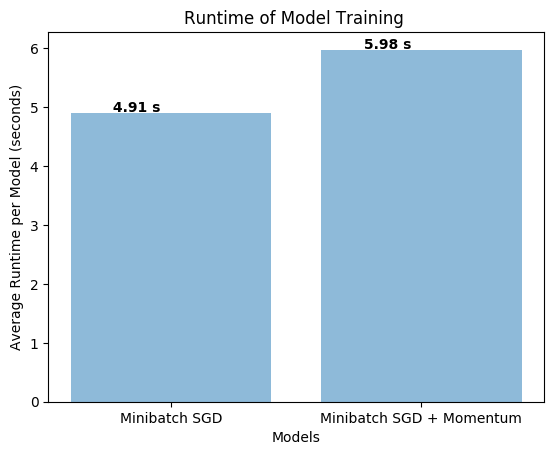
\includegraphics[width=0.45\textwidth]{train_time_part1.png}
\end{center}
\begin{center}
    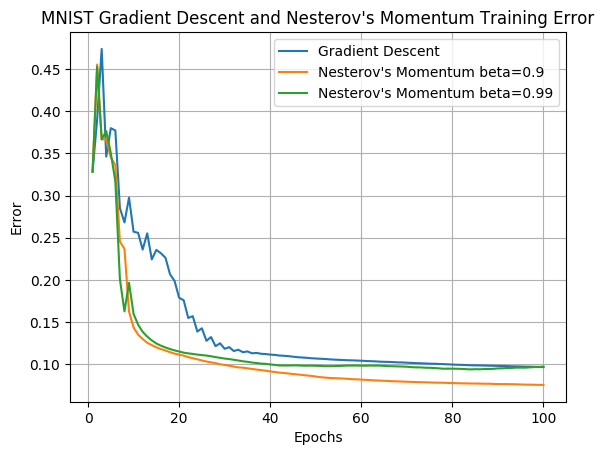
\includegraphics[width=0.45\textwidth]{GradientDescentandNesterov'sMomentumTrainingError.png}
\end{center}
\begin{center}
    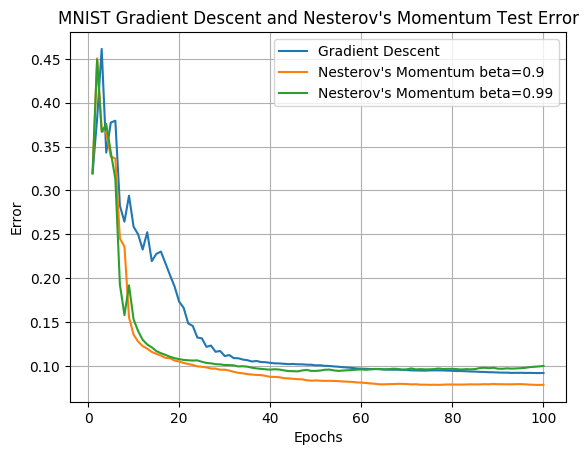
\includegraphics[width=0.45\textwidth]{GradientDescentandNesterov'sMomentumTestError.png}
\end{center}
\begin{center}
    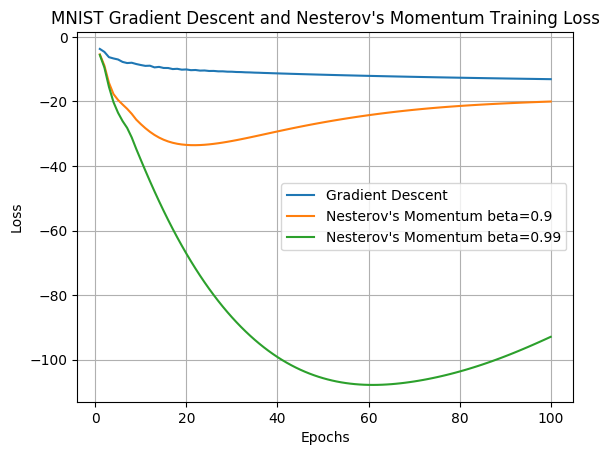
\includegraphics[width=0.45\textwidth]{GradientDescentandNesterov'sMomentumTrainingLoss.png}
\end{center}
We proceeded to explore other combinations of hyperparameters for these two algorithms and compared the outputs. The plots can be seen below.\par
\begin{center}
    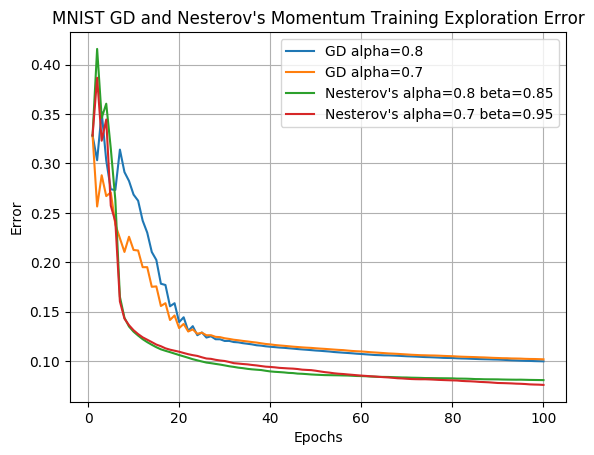
\includegraphics[width=0.45\textwidth]{GDandNesterov'sMomentumTrainingExplorationError.png}
\end{center}
\begin{center}
    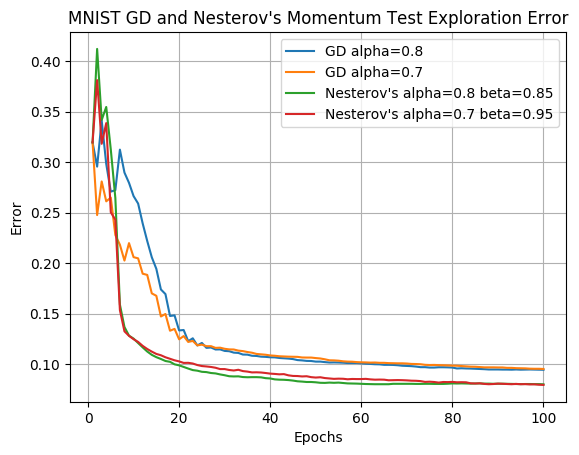
\includegraphics[width=0.45\textwidth]{GDandNesterov'sMomentumTestExplorationError.png}
\end{center}
\begin{center}
    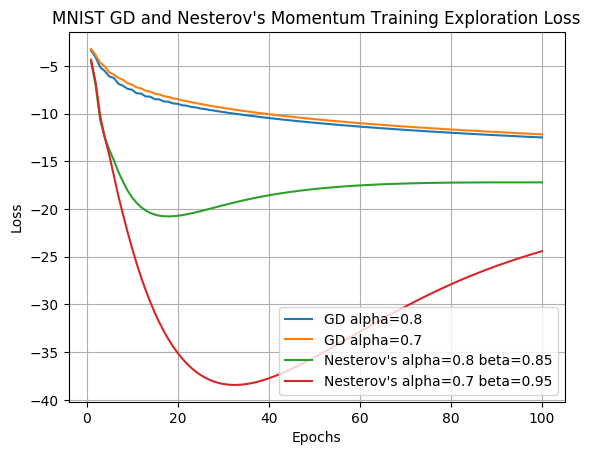
\includegraphics[width=0.45\textwidth]{GDandNesterov'sMomentumTrainingExplorationLoss.png}
\end{center}

\textbf{Part I: Exploration}
\begin{center}
    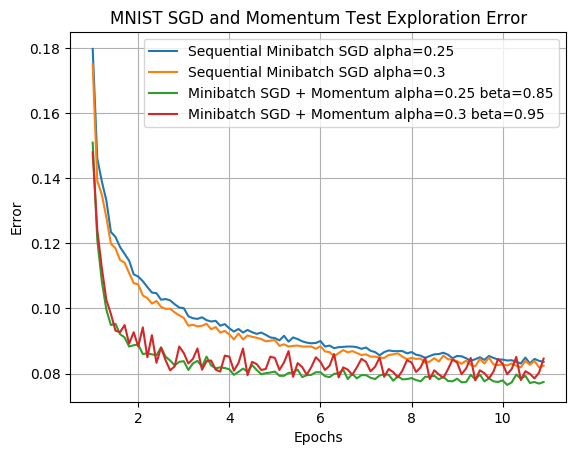
\includegraphics[width=0.45\textwidth]{SGDandMomentumTestExplorationError.png}
\end{center}
\begin{center}
    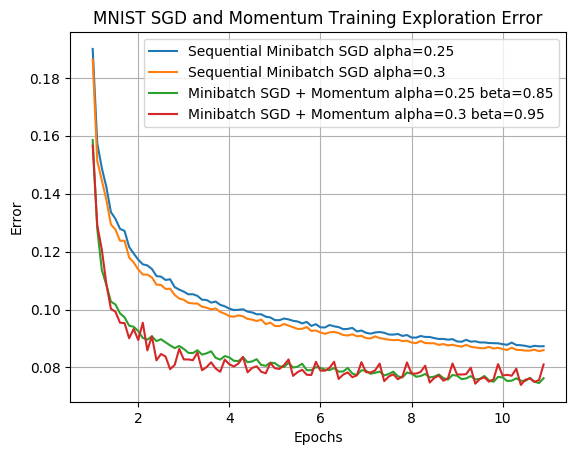
\includegraphics[width=0.45\textwidth]{SGDandMomentumTrainingExplorationError.png}
\end{center}
\begin{center}
    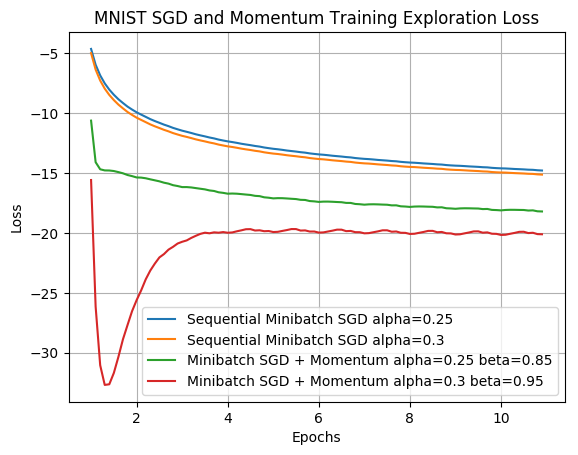
\includegraphics[width=0.45\textwidth]{SGDandMomentumTrainingExplorationLoss.png}
\end{center}
\end{multicols}

\begin{multicols}{2}
\noindent
\textbf{Part II: Momentum and SGD}\par 
I also compared two sequential variations of gradient descent, namely \textit{Sequential Minibatch SGD}, with and without momentum. I ran regular sequential minibatch SGD once, and its modified momentum version twice, once with momentum parameters $\beta=0.9$ and $\beta=0.99$ respectively. All three executions used a step size $\alpha = 0.2$, and went through 10 epochs recording the model parameters every $1/10$ of the epoch (at every full gradient step, with minibatch size $B=600$ on the MNIST training set which contains 60,000 points.\par
The training and test error as well as the cross-entropy loss on the training set were computed and recorded per model update and the plots are shown on the below. Again, the momentum optimization with $\beta=0.9$ outperformed the others, reaching a training and test error of about 8\% while momentum with $\beta=.99$ remained at about 10\% error on the test set and SGD finished at around 9\%. SGD and momentum with $\beta=.99$, on average, did continue to decrease the training and test error through all the 10 epochs, but momentum with $\beta=.9$ was far ahead by the fouth epoch, and still continued to decrese the error rate although rather slowly while regular SGD was slowly catching up. \par
SGD monotonously decreased the loss function throughout training, although rather slowly compared to momentum with $\beta = .99$, which decreased the loss almost an order of magnitude more in the first two epochs, and then started increasing it again although finishing at a much lower value than the others. Momentum with $\beta=0.9$ on the other hand, rapidly decreased the loss over one epoch and then plateaued and finished at a lower loss than SGD.\par
Finally, I also averaged the runtime of both, sequential minibatch SGD and it's momentum counterpart over five runs, each of which completed 10 epochs of training as summarized above. the results are summarized on the plot below: both algorithms ran much faster than their non-minibatch counterparts, reaching lower training and test errors in just 5-6 seconds with the non-momentum version finishing faster.
\begin{center}
    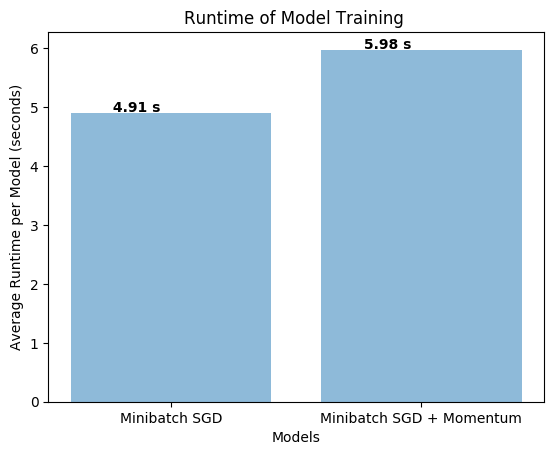
\includegraphics[width=0.45\textwidth]{train_time_part2.png}
\end{center}
\begin{center}
    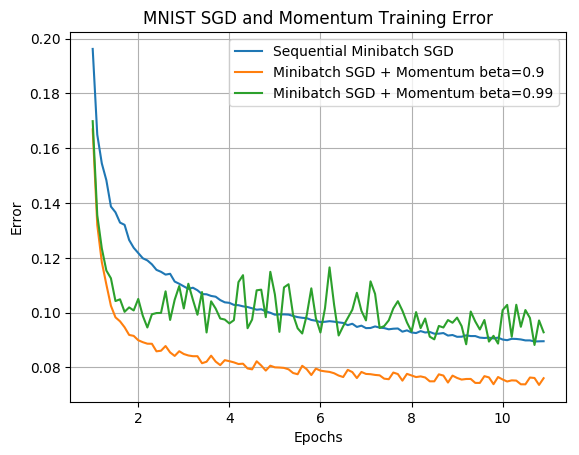
\includegraphics[width=0.45\textwidth]{SGDandMomentumTrainingError.png}
\end{center}
\begin{center}
    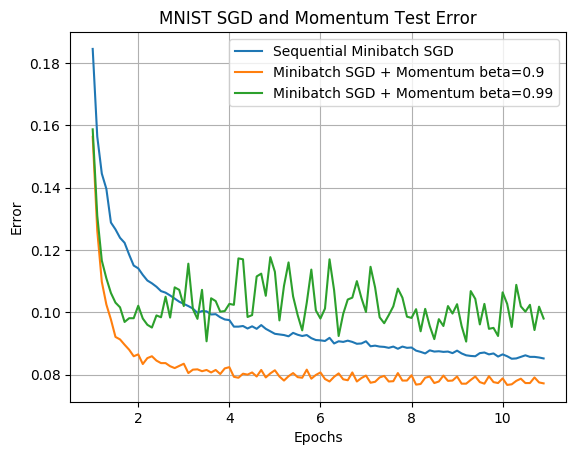
\includegraphics[width=0.45\textwidth]{SGDandMomentumTestError.png}
\end{center}
\begin{center}
    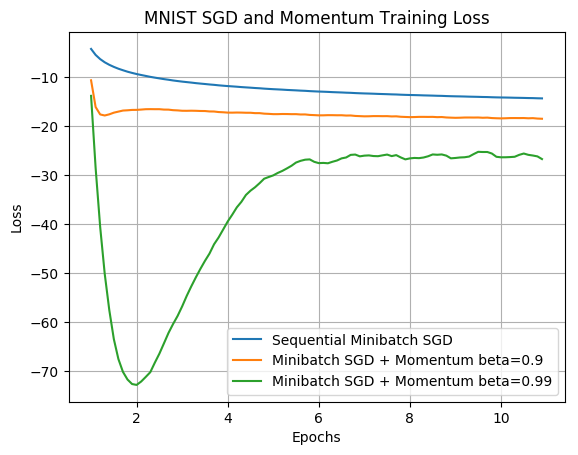
\includegraphics[width=0.45\textwidth]{SGDandMomentumTrainingLoss.png}
\end{center}
\noindent
\textbf{Part II: Exploration} \par
A few more settings of $\alpha$ and $\beta$ were tested, and the plots of the training and test errors, as well as the cross-entropy loss on the training set are plotted below for each of the optimizations. Over all these parameter settings, SGD with momentum still performs better, with $\beta=.85$ bringing the test error below 8\%. The sequential algorithms are rather close, nonetheless, giving a comparable test error to that of the rather noisy momentum run with $(\beta=.95)$. The non-momentum optimizers slowly and monotonously decrease the loss over all training, while $(\beta=.85)$ decreased it tremendously over the first epoch and then increased also quite a lot. On the other hand, $(\beta=0.85)$ behaves quire similarly to $(\beta=.9)$ from the previous section.
\begin{center}
    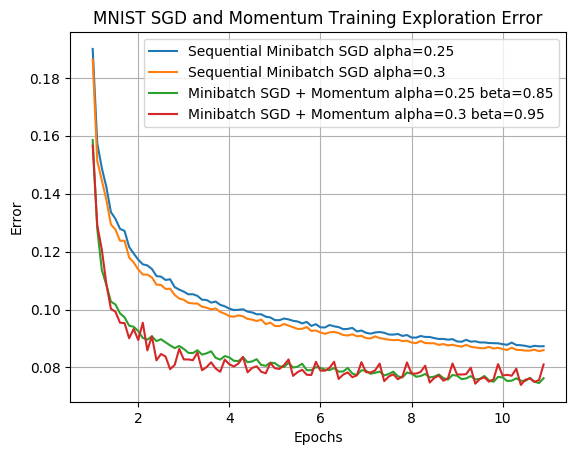
\includegraphics[width=0.45\textwidth]{SGDandMomentumTrainingExplorationError.png}
\end{center}
\begin{center}
    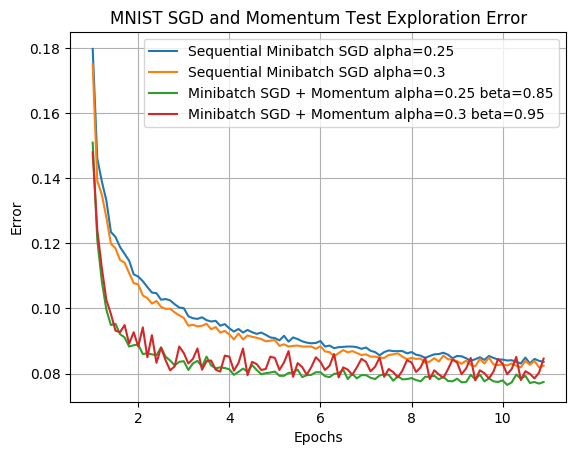
\includegraphics[width=0.45\textwidth]{SGDandMomentumTestExplorationError.png}
\end{center}
\begin{center}
    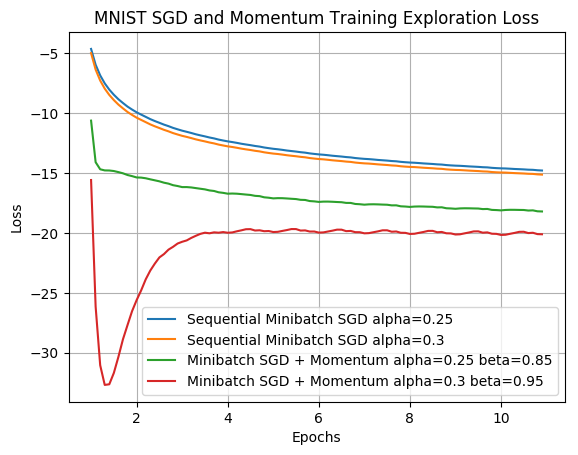
\includegraphics[width=0.45\textwidth]{SGDandMomentumTrainingExplorationLoss.png}
\end{center}

\textbf{Part III: ADAM}
Finally, I also compared our old friend, \textit{Sequential Minibatch SGD} with the grandfather of adaptive algorithms, \textit{ADAM}. I executed another independent run of SGD to the one shown in Part II, with $\alpha = 0.2$ over 10 epochs, computing the training and test error as well as the value of the loss function on the training set 10 times per epoch. ADAM was executed in a similar fashion, but using step size $\alpha0.01$ and respective first and second decay rates $\rho_1 = 0.9$ and $\rho_2 = 0.999$. The results are summarized in the plots below.\par 
ADAM is able to bring the training and test error down, at an incredibly fast rate over the first epoch (at least comparatively), but the test error slows down and almost plateaus right away as well. In fact, it would seems as thought the training error for ADAM is just the training error for SGD shifted down by two percent, but we can see that the same does not hold for the test error. Nonetheless, the test error is still about 1\% smaller for ADAM than it is for SGD. \par
The training losses, just like the training errors, have extremely similar shapes, but ADAM's is shifted down. In addition, both SGD and ADAM monotonously bring the loss down, unlike SGD with momentum as was previously shown. \par 
I also measured the runtime for both algorithms, but now over a total of 15 independent executions since the results seemed to vary largely. Both algorithms performed comparatively, with SGD being only slight faster at about 5.2:5.8 seconds. This is great news, if there's any time constraints, we could just run ADAM since it seems like for any allotted time $\Delta t$ at which SGD might give reasonable good results, ADAM is likely to perform better by the plots below.\par
\begin{center}
    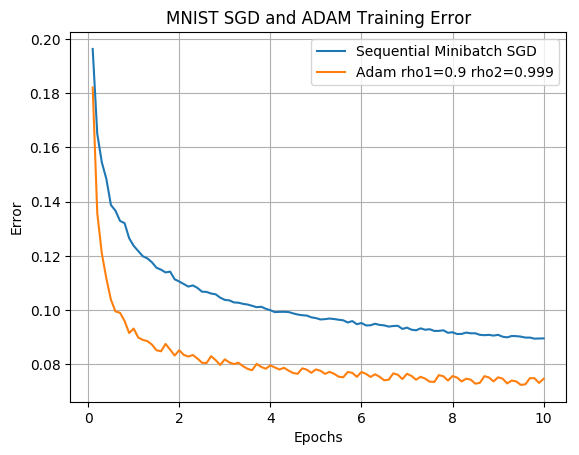
\includegraphics[width=0.45\textwidth]{SGDandADAMTrainingError.png}
\end{center}
\begin{center}
    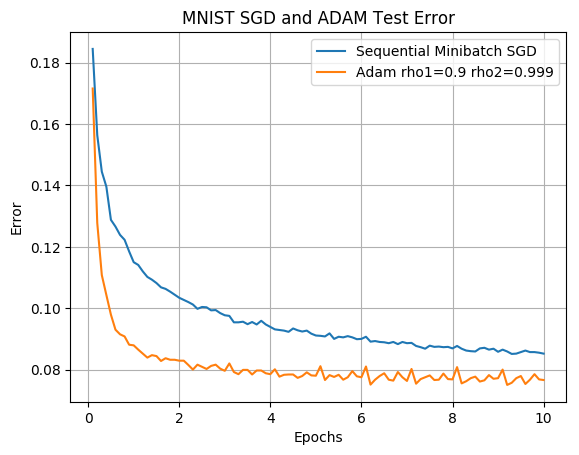
\includegraphics[width=0.45\textwidth]{SGDandADAMTestError.png}
\end{center}
\begin{center}
    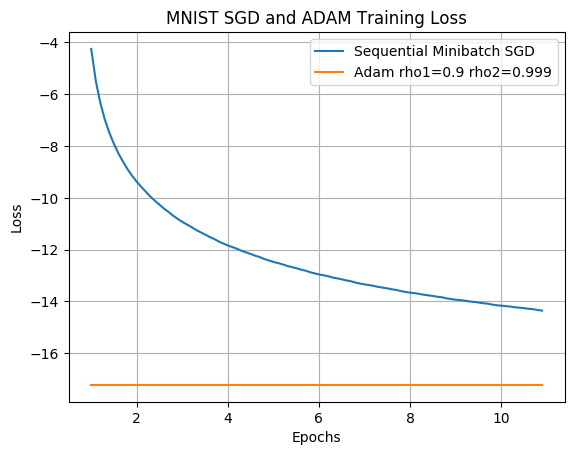
\includegraphics[width=0.45\textwidth]{SGDandADAMTrainingLoss.png}
\end{center} 

\begin{center}
    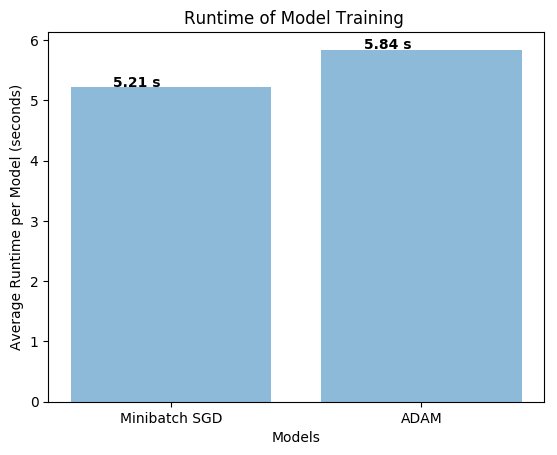
\includegraphics[width=0.45\textwidth]{train_time_part3.png}
\end{center}
\noindent
\textbf{Part II: Exploration} \par
I explored other settings of $\alpha$ and $\beta$ that would give reasonable accuracy. I reused the values of $\alpha$ from the exploration in Part II, and used the decay parameters listed in the figures. As we would expect, ADAM performed better for any of the four parameter settings tested. Interestingly, as shown on the plots, all four parameter settings performed very similarly on the test set, although the loss functions behave slightly differently (they are all, to a reasonable approximation, vertical shifts of one another). Each run of ADAM behave more similar to the other run that used the same $\alpha$, which suggests that determining a good value for $\alpha $ is still very important. In terms of accuracy and runtime, then, ADAM seems like the clear winner.\par

\begin{center}
    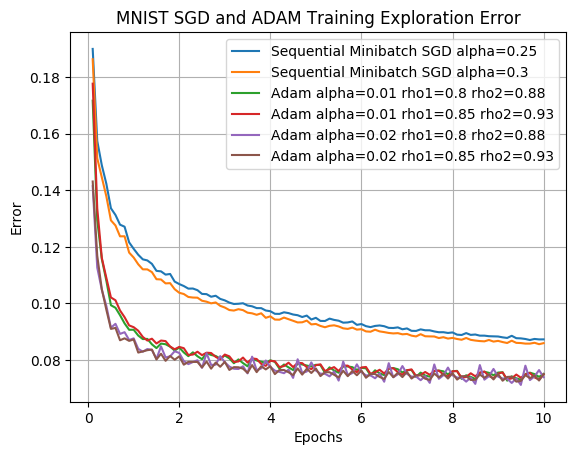
\includegraphics[width=0.45\textwidth]{SGDandADAMTrainingExplorationError.png}
\end{center}
\begin{center}
    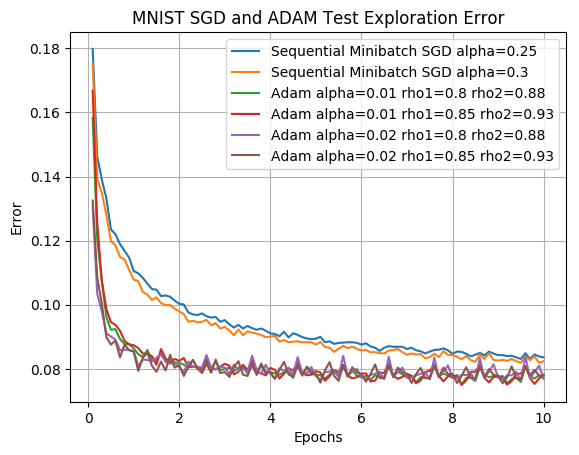
\includegraphics[width=0.45\textwidth]{SGDandADAMTestExplorationError.png}
\end{center}
\begin{center}
    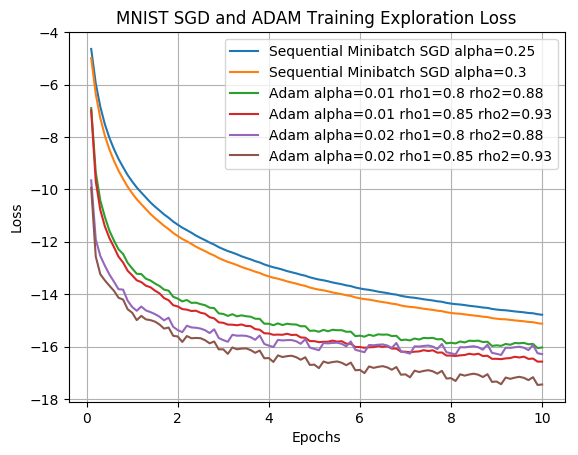
\includegraphics[width=0.45\textwidth]{SGDandADAMTrainingExplorationLoss.png}
\end{center}
\end{multicols}




\end{document}
